\documentclass[a4paper, 12pt]{article}
% \usepackage[a4paper, total={7in, 8in}]{geometry}
\usepackage{graphicx}
\usepackage{subfigure}
\usepackage{multicol}
\usepackage{amsmath}


\usepackage[english]{babel}
\usepackage[noheader]{packages/sleek}
\usepackage{packages/sleek-title}
\usepackage{packages/sleek-theorems}
\usepackage{packages/sleek-listings}


    
% \logo{title.png}
    \institute{\huge{Habib University}}
    \faculty{CS/SDP 262 Computational Social Science \\
    Fall 2020}
    \title{Agent Based Modelling of Slime Mold}
    \subtitle{Submitted to: Dr. Shah Jamal Alam}
    \author{\Large{\textit{Authors:} Ali Hamza; Bahzad Badvi; Muhammad Usaid}}
    \date{\today}
    
%%%%%%%%%%
% Others %
%%%%%%%%%%

\lstdefinestyle{latex}{
    language=TeX,
    style=default,
    %%%%%
    commentstyle=\ForestGreen,
    keywordstyle=\TrueBlue,
    stringstyle=\VeronicaPurple,
    emphstyle=\TrueBlue,
    %%%%%
    emph={LaTeX, usepackage, textit, textbf, textsc}
}

\FrameTBStyle{latex}

\def\tbs{\textbackslash}

%%%%%%%%%%%%
% Document %
%%%%%%%%%%%%
    
    
\begin{document}
\maketitle
\newpage
\tableofcontents
\newpage
\section{Introduction}
\subsection{Abstract}
Anthropocentrism and the capitalistic commodification of resources has led humans down a spiral of self-destruction, and equally increased a general disregard for nature. For most nature is an external entity, unbeknown to them that humanity is not exclusive from it. Following from this stems the negligence of intelligence shown in nature however, as we shall be exploring in our project, signs of intelligence can be found everywhere in nature. Our project deals with modelling the semi-intelligent behavior shown by a cellular organism known as Physarum Polycephalum or more commonly as Yellow slime mold. This organism has baffled biologist and researcher over its exhibition of intelligence besides the fact that it does not have a central nervous system. Surely without a central processing unit how can an organism function let alone solve difficult problems? Intriguingly enough P.Polycephalum cannot only perform basic life function but is able to solve many complex problems such as path optimization. Research suggest that a pulsating flow of biochemicals within its tube-like structure handles P.Polycephalum’s intricate mobility and that the control of this fluid is the cause of its coordinated growth. Another research suggests that P.Polycephalum makes use of an external ‘spatial’ memory by using pheromones to mark visited regions.\par 
\textbf{Github}: \url{https://github.com/hurryingauto3/CS262-Computational-Social-Science}

% \subsection{Purpose}
% We are studying \textit{Physarum polycephalum} in the context of an agent-based model because it will allow us to better understand its situational behavior. By implementing an agent-based model we can think about the behavior of P. polycephalum in algorithmic terms. It will also allow us to introduce different parameters and observe the changes in the behavior based on those parameters.

\subsection{Approach}

To try and obtain a holistic understanding and to model the behavior of P. polycephalum with a reasonable degree of accuracy, we will be using two different agent based models - each with a separate goal. The first ABM attempts to model the behavior of the slime mold as it coalesces around food sources in a maze. The maze is generated randomly and slime mold nuclei are randomly distributed across the maze and then are linked. The ABM intends to model the primitive behavior that the mold exhibits - it moves closer and closer to the food source, while the nuclei away from the food source tend to die off. However in doing so, it effectively solves the maze. 

The second agent based model we implemented attempts to explore the problem solving behavior of the P. polycephalum. Our motivation behind this was found in Rules for Biologically Inspired Adaptive Network Design. Slime mold replicated the Tokyo rail network - solving a complex compuational problem with seemingly very little intelligence. Therefore, we wanted to explore how this behavior comes about.        
\newpage
\section{Technical Documentation }
\subsection{Agent Based Model 1}

\begin{enumerate}
    \item \textbf{Name: } \texttt{Maze Solving Simulation via Replication of Slime Mold Behavior}
    \item \textbf{Purpose}\par 
    Using an agent-based model allows us to explore how the agents (nuclei) react with the surroundings and how they can adapt to randomized mazes and find an optimal solution. We cannot model slime mold using a simple algorithmic approach.  
    
    \item \textbf{Agents}
        \begin{enumerate}
        \item Turtles - represent the P. Polycephalum nuclei
        \begin{enumerate}
        \item \texttt{distfood} - The Euclidean distance from the nucleus to the food source stored as an attribute for Agents.
        
        \end{enumerate}
        \item Links - represent the tubular connectivity between the nuclei
        \begin{enumerate}
            \item \texttt{midptx}, \texttt{midptx1}, \texttt{midptx2} - The x-coordinates of three midpoints of a link stored as an attribute for links. 
        \item \texttt{midpty}, \texttt{midpty1}, \texttt{midpty2} - The y-coordinates of three midpoints of a link stored as an attribute for links.
        \end{enumerate}
        \item Patches - represent paths and walls in the maze 
            \begin{enumerate}
                \item \texttt{pcolor}: Black patches are paths; White patches are walls. 
            \end{enumerate}
             
        \item \textbf{Time}\par
        In reality Slime mold grows at about a centimeter an hour so it’s ideal to have the time scale of one tick being equal to an hour. Anything less would be redundant. In our environment we've made it as such so that a step of $0.3$ is equivalent to a step of $1 cm$ in a real-world scenario.
    \end{enumerate}
    
    
    \item \textbf{State/Global Variables}
    \begin{enumerate}
        \item \textbf{Global Variables}:
    \begin{enumerate}
        \item \texttt{Left-Height} - Represents \texttt{pycor} for the start food source (patch with red color)
        \item \texttt{Right-Height} - Represents \texttt{pycor} for the end food source (patch with red color)
        \item \texttt{prob\_random} - Represents the probability that a nucleus would move randomly, lies within the range $0$ and $1$ and the default value is $0.6$
        \item \texttt{prob\_static} - Represents the probability that a nucleus would remain static, lies within the range $0$ and $1$ and the default value is $0.6$
        \item \texttt{prob-reproduce} - Represents the probability that a nucleus divides creating another,lies within the range $0$ and $1$ and the default value is $0.15$
        \item \texttt{num-agents} - Represents the number of initial nuclei in the model, lies in range $0$ to $6000$ default value is $1000$
        \item \texttt{sumfooddist} - Represents the sum of distances of nuclei from a food source.
    \end{enumerate}
    \end{enumerate}
    
    \item \textbf{Process Overview and Scheduling:} 
    
    %\begin{enumerate}
        %\item If nuclei are on the white patch, make them die. 
        %\item Make nuclei move on black patches while making them face their linked neighbors. 
        %\item If there are no neighbors, make agents move based on \texttt{prob\_random}.
        %\item Update distance of nucleus and food source. 
        %\item Check edges and then remake them to make sure they follow rules.
        %\item Make nuclei reproduce using \texttt{prob-reproduce}.
        %\item Stop when ticks = 50.
    %\end{enumerate}
    
        \textit{Following actions take place every time step (hour):}
    \begin{itemize}
        \item For each agent draw a random-float between 0 and 1 to check if \texttt{prob\_static} is achieved or if agent is on a food source.
        \begin{itemize}
            \item If above mentioned condition is achieved do nothing
            \item Else store a link-neighbor which is closest to any randomly chosen food source (could be both start or finish) in a local variable called \texttt{face-to}. If \texttt{face-to} is equal to nobody or a random-float in range 0 to 1 is within \texttt{prob\_random} face any randomly chosen link-neighbor else face the agent stored in \texttt{face-to}. Move one centimeter (that is equivalent to \texttt{fd 0.3} in our case) if the topology of the maze allows for it.
        \end{itemize}
        \item Then call the following procedures: 
        \begin{itemize}
            \item \texttt{foodupdate}
            \item \texttt{make-edges}
            \item \texttt{reproduction}
        \end{itemize}
    \end{itemize}
    
    \item \textbf{Sensing}\par
    The agent's movement is such that in each step they either move randomly, remain static, or they move towards a neighbor which is closer to the food node. The movement of an agent towards their neighbor is motivated from the fact that the nuclei prioritizes movement towards the direction it's obtaining the greatest nutrition hence an assumption is made that the flow of nutrients from the neighbor closest to the food source would be greater.
    
   \item \textbf{Interaction}\\
   Each agent is connected with another agent via a link these links are thence contribute to the movement the agents make throughout the simulation as discussed.
    
     \item \textbf{Stochasticity/Randomness} \par
    \textit{Randomness occurs in the following ways}:
    \begin{enumerate}
        \item The maze generation is done randomly and has been taken from:\\ \url{http://ccl.northwestern.edu/netlogo/models/community/BAM20Maze20Generator2)}
        \item Locations of agents which are generated to represent the nuclei are set to a random coordinate
        \item Normally (that is when \texttt{prob\_random} and \texttt{prob\_static} is not achieved) when an agent chooses which connected neighbor to face and move towards, the selection is done randomly from two choices:
        \begin{enumerate}
            \item A link-neighbor closest to the starting food node
            \item A link-neighbor closest to the ending food node
        \end{enumerate}
        \item A random-float is usually generated to check if probabilities \texttt{prob\_random}, \texttt{prob\_static} are achieved
        \item Once \texttt{prob\_random} is achieved the agent may face in any random direction and take a step
        \item A random-float is used to compare the value of the number with the variable \texttt{prob-reproduce} to determine whether a nucleus would divide, therefore the reproduction action relies on randomness.  
        \item If the topology doesn't allow for a newly generated agent to be placed nearby parent agent, the newly generated agent is placed at a randomly selected coordinate in the environment.
    \end{enumerate}
    
    
    \item \textbf{Setup and Initialization}
    \begin{enumerate}
        \item \textbf{Environment}\par
        The environment is a geo-spacial environment where we can setup mazes/walls to show how P.Polycephalum is able to overcome such scenarios.
        \item \textbf{Turtles/ Links/ Patches}
        \begin{enumerate}
            \item \texttt{setup-maze, setup-start-finish, make-maze} is used to create the maze at the start. (Details of these processes can be referred from BAM's maze generation model inspired from \url{http://ccl.northwestern.edu/netlogo/models/community/BAM20Maze20Generator2)}
            \item Create \texttt{num-agents} number of nuclei and then place them randomly around the world. 
            \item Delete all nuclei that are created on a wall (white patch). 
            \item Update distance of the nuclei from the nearest food source.
            \item Create links between nuclei.  
        \end{enumerate}
    \end{enumerate}
    \item \textbf{Input Data} \par
    This ABM does not take any input.
    \item \textbf{Outputs} \par
    Plots display the number of turtles and the average distance from food source (\texttt{sumfooddist / count turtles}).
    
    \item \textbf{Sub models and Processes}
    \begin{enumerate}
        \item \texttt{setup-maze, setup-start-finish, make-maze} (Details of these processes can be referred from BAM's maze generation model inspired from \url{http://ccl.northwestern.edu/netlogo/models/community/BAM20Maze20Generator2)}
        \item \texttt{kill} - This process is used to kill the maze-making agents once the maze is constructed
        \item \texttt{add-nuclei} - This process adds \texttt{num-agents} number of agents in the environment at random co-ordinates and then removes those which are generate on a wall. The agents created by this process are the abstraction of P.Polycephalum's nuclei. This procedure then calls \texttt{foodupdate} and \texttt{make-edges}
        \item \texttt{foodupdate} - This process updates the distfood for each agent by storing the euclidean distance to the closest food source.
        \item \texttt{make-edges} - This process connect each agents with $15$ agents which are closest to it and are not already connected. Once linking is done this process also checks if a link is crossing over a wall using \texttt{midptx}, \texttt{midptx1}, \texttt{midptx2}, \texttt{midpty}, \texttt{midpty1}, and \texttt{midpty2}, if so that link is terminated. Lastly any agent which is left with no \texttt{link-neighbor} is killed.
        \item \texttt{reproduction} - Every $4$ ticks this process ask $100$ randomly selected agents with their \texttt{distfood} within \texttt{sumfooddist / count turtles} to produce another nuclei if a randomly generated number falls within the prob-reproduce and locate them nearby the parent agent if topology allows else set the coordinates randomly.
        \end{enumerate}
    \end{enumerate}
    \newpage

    \begin{figure}[h!]
        \centering
        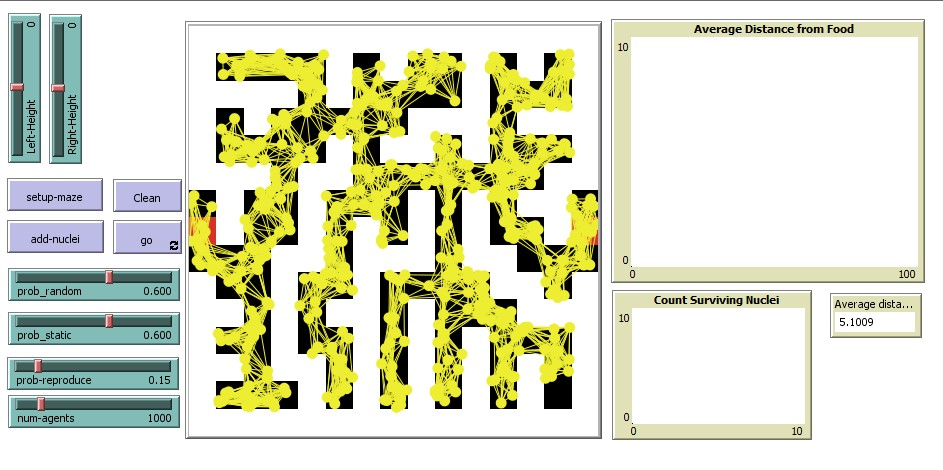
\includegraphics[scale = 0.67]{Images/abm1_start.jpg}
        \caption{Start state of ABM 1}
        \label{fig:abm1start}
        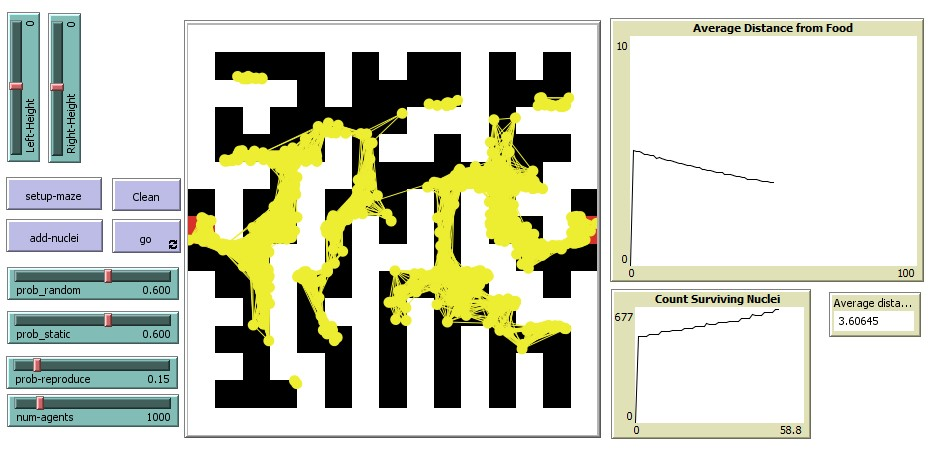
\includegraphics[scale = 0.67]{Images/abm1_end.jpg}
        \caption{End state of ABM 1}
        \label{fig:abm1end}
    \end{figure}
    \newpage
\subsection{Agent Based Model 2}
    
\begin{enumerate}
    \item \textbf{Name: }\texttt{ Minimum Spanning Graph Simulation via Replication of Slime Mold Behavior}
    \item \textbf{Purpose}: Since there isn't a mathematical model that can be used to explain the behavior of slime mold, agent-based modelling can be used. Although the agents are homogeneous, they interact with the environment around them to find solutions to problems related to food sources, for example, finding an optimal path between multiple food sources.  
    \item \textbf{Agents}\par
    \begin{enumerate}
        \item Turtles - represent the P. Polycephalum nuclei
        \item Links - represent the tubular connectivity between the nuclei
        \item Patches - represent physical space of the world 
            \begin{enumerate}
                \item \texttt{trail-val}: The measure of food chemicals on a certain patch.
                \item \texttt{is-food?}: A Boolean value that tells whether a patch is a food patch or not.
            \end{enumerate}
        \item \textbf{Time} - Each tick represents an hour.
    \end{enumerate}
    \item \textbf{State/Global Variables}
    \begin{enumerate}
        \item \textbf{Global Variables}
        \begin{enumerate}
            \item \texttt{num-food-nodes}: The number of patches that are a food source. It lies within 0 and 60 and has a default value of 11. 
            \item \texttt{angle-vision}: It lies within 0 and 100 and has a default value of 30. 
            \item \texttt{num-nuclei}: The number of slime mold nuclei in the experiment, ranging from 0 to 5000 and having a default value of 900.
            \item \texttt{food-secrete}: The amount of chemicals released by a food patch, ranging from 0 and 10, with a default value of $3.7$.
            \item \texttt{step}: It represents how much a nucleus would move in a tick. It lies between 0 and 2 and has a default value of $1.0$.
            \item \texttt{evaporation-rate}: The rate at which the food chemicals evaporate on a patch, ranging from 0 to 1 and having a default value of 0.1. 
            \item \texttt{turtle-secrete}: The amount of chemicals left by a turtle (nucleus) on a patch, ranging from 0 to 10 and having a default value of 0.6. 
        \end{enumerate} 
    \end{enumerate}

    
    \item \textbf{Process overview and Scheduling} 
    \begin{enumerate}
        \item Make the turtles move. 
        \item Update the chemical trail each tick.
        \item After the tick, delete existing edges. 
        \item Create edges again between the nuclei. 
       \end{enumerate} 
        These processes are further explained in point 12 below. 
    
    \item \textbf{Sensing} \\
    The nuclei can pick up food chemicals that are left by food sources and by other nuclei. They can do so only within a set angle of vision determined by \texttt{angle-vision}. 
    \item \textbf{Interaction} \\
    The slime mold nuclei are connected with each other using links. The nuclei interact with patches which determines their movement, which is expounded upon below.  
    
   
    \item \textbf{Stochastic/Randomness } 
    \begin{enumerate}
        \item The patches that are food sources are assigned randomly based on the value of \texttt{num-food-nodes}.
        \item The positions of the nuclei - the \texttt{x} and \texttt{y} coordinates - also assigned randomly.
    \end{enumerate}
    \item \textbf{Setup and Initialization}
    \begin{enumerate}
        \item \textbf{Environment}:  This model uses a geo-spatial, wrapped environment that represents an abstract 2D space where the slime mold can interact with the food.
        \item \textbf{Turtles/ Links/ Patches}
        \begin{enumerate}
            \item Default Number of Turtles = 900
            \item The turtles are connected with 5 other turtles in the shortest distance via links
            \item The patches are initialized with \texttt{trail-val} = 1 and randomly sets \texttt{is-food?} = \texttt{true} for \texttt{num-food-nodes} patches 
        \end{enumerate}
    \end{enumerate}
   
    \item \textbf{Input Data} \\
    This ABM does not take any inputs. 
    
    \item \textbf{Outputs} \\
    This ABM does not give any quantitative output. It gives a visual representation of a minimum-spanning tree formed by the nuclei and the food nodes. 
    \item \textbf{Sub models and Processes}
    \begin{enumerate}
    \item \texttt{move} - This sub process determines the movement of each turtle based on the above mentioned global variables
    \item \texttt{update-secretion} - This sub process updates the chemical trail values on each patch and changes their colors accordingly.
        \item \texttt{del-edges} - This sub process is called at every tick and it deletes previous links that are no longer the shortest length links.
        \item \texttt{make-edges} - This sub process is called at every tick to create new links of minimum distance between each turtle and 5 other turtles
    \end{enumerate}
    \end{enumerate}
   \newpage

    \begin{figure}[h!]
        \centering
        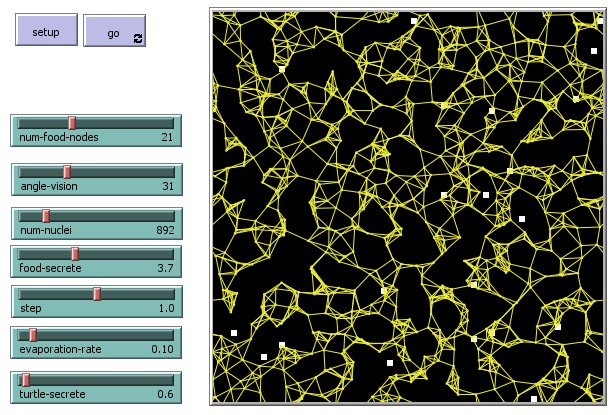
\includegraphics[scale = 0.67]{Images/abm2_start.jpg}
        \caption{Start state of ABM 1}
        \label{fig:abm2start}
        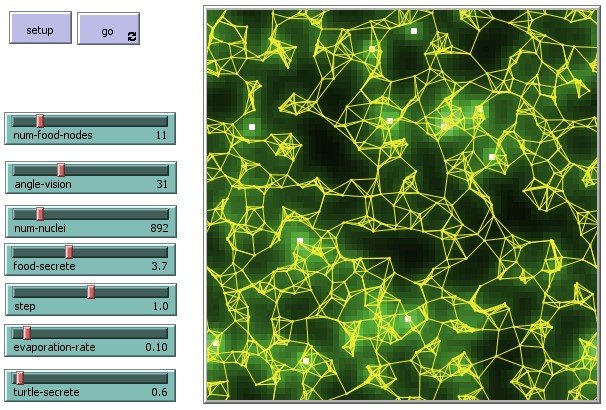
\includegraphics[scale = 0.67]{Images/abm2_end.jpg}
        \caption{End state of ABM 1}
        \label{fig:abm2end}
    \end{figure}
    \newpage
\section{Analysis of Data}
Since, the primary goal of this project was an inquiry into the inner workings of the slime mold, we chose to not limit our study to just using ABM's. Through the use of the ABM we built that is referenced in section 2.1 we were able to acquire 3 independent variables that could be used to model the slime mold, and predict its decisions. We did this by using the BehaviorSpace tool present in Netlogo 6.1. We set out a range of changes in the independent variables that we were interested in to see how these changes impact the final average euclidean distance from the two food sources. The experiment was setup as follows: 
\begin{center}
    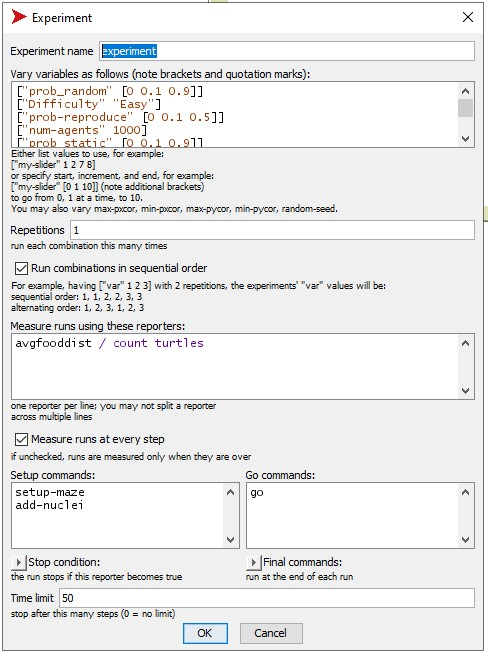
\includegraphics[scale=0.9]{Images/behaviorspace.jpg}
\end{center}
\newpage

We were able the run the experiment twice and obtained 920 data points, which we then analysed using Python, and some libraries. Through this we were able to obtain visualization between the 3 independent variables and the dependent variable. However, the visualizations were very not able to tell us much about how the variables were affecting the final average food distance as the Netlogo model varied multiple quantities simultaneously. This led us to conducting a multivariate least squares regression analysis of the data. This resulted in an equation to predict the final average food distance as follows:
\begin{multline*}
        Final Avg. Food Dist = 1.8157 + 2.4967\cdot P(Random Movement) -\\ 1.7596\cdot P(Reproduction) + 1.2086\cdot P(Static)
\end{multline*}
We were also able to obtain other useful statistical data from the data set that has been summarized on the next page however, we did not further investigate the data as that it was beyond the scope of the project. 

\begin{figure}[h!]
\centering
\subfigure[]{
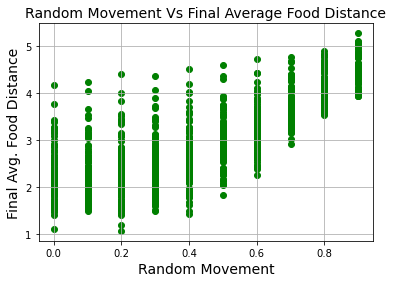
\includegraphics[width=0.40\textwidth]{Images/rndmove.png}
}
\subfigure[]{
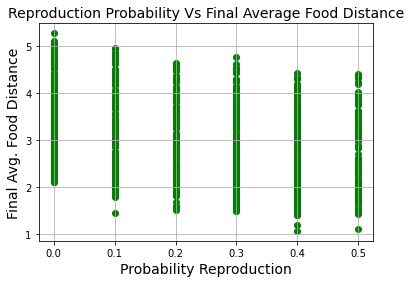
\includegraphics[width=0.42\textwidth]{Images/rndprod.png}
}

\subfigure[]{
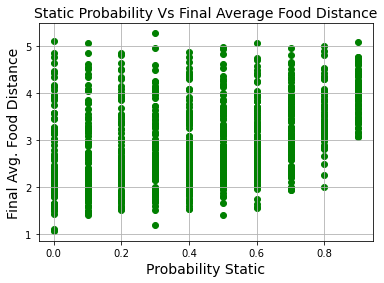
\includegraphics[width=0.45\textwidth]{Images/rndstatic.png}
}
\caption{Scatter Plots of 3 Independent Variables against the Dependent Variable}
\label{fig:Graphs}
\end{figure}
\begin{center}
    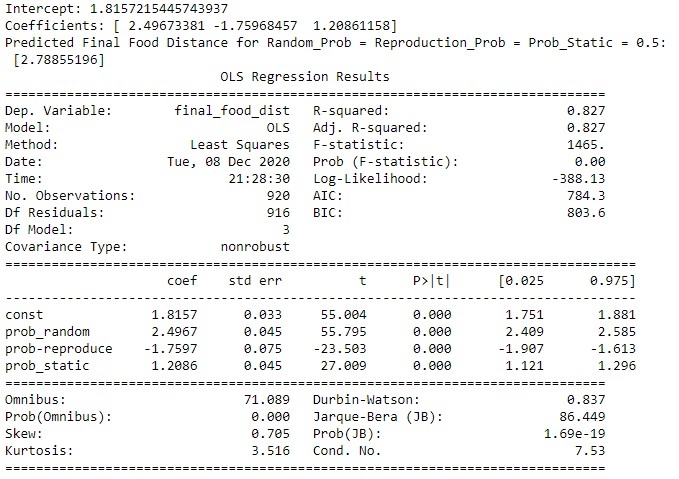
\includegraphics[scale = 0.9]{Images/data.jpg}
\end{center}
\newpage
\section{Limitations of the Model}
\subsection{Computational Limitations}
Since, our project was focused on an organism that has trillions of of nuclei, we knew computational complexity would be a problem for us from the start. We tried to explore avenues of incorporating multi-threading or perhaps use the CUDA cores of the discrete GPUs in our machines but that required the usage of another ABM modelling software called, Flame GPU. This was, obviously, outside the defined scope of the project so we were unable to rectify this issue.
\subsection{Linking the Nuclei}
Another major challenge was to ensure that links were being formed properly. We had to make sure that the links between two nuclei do not cross over a wall in the maze (a white patch). We simulated the slime's inability to create linkages through walls by simulating only links that were not crosses the wall. We calculated the 3 midpoints across each link and if any of those were intercepting the $x$ and $y$ coordinates of a white patch, we would eliminate the links. This added another layer layer of computational complexity within the model which furthered the limitations of the computational aspects of our ABM. 
\subsection{Preventing Clustering}
Another challenge was the fact that clusters form in areas in the maze. Theoretically, these clusters should die because they get stuck and cannot access food source, and are disconnected from the rest of the P.Polycephalum. Unfortunately, eliminating these clusters would be very computationally expensive - which means that its more effective to let them be for the sake of practicality of the model, since the model itself is also computationally expensive due to the large number of nuclei and links that need to be iterated very often.  

\subsection{Lack of Pre-existing Research}
A difficulty that we faced was the fact that there does not exist a lot of reasearch on the computational aspect of P. polycephalum. It was difficult to try and emulate a deterministic biological aspect into a probabilistic model in order to emulate the behavior of the slime mold. Availibility of more quantitative research would have helped us to think algorithmically about its behavior, but unfortunately that was difficult for us to do.   
\newpage
\section{Conclusion}
It would be unfair to say that this study in the behavior of the very titular slime mold, P.Polycephalum, via Agent Based Modelling has been conclusive. However, it is important to understand that it has provided us new insights, and questions, about its mechanism. We explored the slime mold using two Agent Based Models that tested out two different phenomena the slime mold has shown in the real world. 1) Its ability to solve mazes with food particles at the start and the end. 2) Its ability to form highly optimized paths between many food particles. \par 
It is apparent that recreating the behavior of the slime mold is a highly difficult task due to the lack in substantial information present about its inner workings, a very important aspect that is required in algorithmic; deterministic processes. However, the use of ABM's has proven to be quite useful in allowing us to circumvent this limitation via the ability to introduce stochastic measures within the world that the potentially correct model of the slime mold can then react to. The simulations of these ABMs have provided us great insights as to how the slime mold \textit{may} react in various conditions.
\par 
Moreover, our models were not able to completely do justice to the slime mold as it is much more optimized than our models that we produced but we were able to create data points from the model and create a least squares regression of the slime molds position with respect to 3 data points. However, we must understand that the model can incorporate many more data points to predict better positional changes in the slime mold but such a model was out of the scope of this study.
\par 
The slime mold seems to have great potential in being able to solve various graph theory problems as we have observed but to be able to replicate its processes requires much more research into its behaviors from a computational perspective at this point in time.
\newpage
\section{Bibliography}

\begin{enumerate}
    \item Alim, K., Amselem, G., Peaudecerf, F., Brenner, M., & Pringle, A. (2013). Random network peristalsis in Physarum polycephalum organizes fluid flows across an individual. Proceedings of the National Academy of Sciences of the United States of America, 110(33), 13306-13311. Retrieved September 12, 2020, from \url{http://www.jstor.org/stable/42712903}
    \paragraph{}
    \item Alim, K., Andrew, N., Pringle, A., Brenner, M. (2017). Mechanism of signal propagation in Physarum polycephalum. Proceedings of the National Academy of Sciences. Retrieved September 12, 2020, from  \url{https://www.pnas.org/content/114/20/5136.short.}
    \paragraph{}
    \item Nakagaki, T., Yamada, H. & Tóth, Á. Maze-solving by an amoeboid organism. Nature 407, 470 (2000). \url{https://doi.org/10.1038/35035159}
    \paragraph{}
    \item Reid, C., Latty, T., Dussutour, A., & Beekman, M. (2012). Slime mold uses an externalized spatial "memory" to navigate in complex environments. Proceedings of the National Academy of Sciences of the United States of America, 109(43), 17490-17494. Retrieved September 12, 2020, from \url{http://www.jstor.org/stable/41829697}
    \paragraph{}
    \item Tero, A., Takagi, S., Saigusa, T., Ito, K., Bebber, D., Flicker, M., . . . Nakagaki, T. (2010). Rules for Biologically Inspired Adaptive Network Design. Science, 327(5964), new series, 439-442. Retrieved September 13, 2020, from \url{http://www.jstor.org/stable/40508592}
    \paragraph{}
    \item Becker, Matthias (2011). [IEEE 2011 IEEE Congress on Evolutionary Computation (CEC) - New Orleans, LA, USA (2011.06.5-2011.06.8)] 2011 IEEE Congress of Evolutionary Computation (CEC) - Design of fault tolerant networks with agent-based simulation of Physarum polycephalum. \url{http://10.1109/CEC.2011.5949630}
\end{enumerate}


\end{document}